\section{Synthesis and Research Gap Analysis}
\label{sec:synthesis_gap}

The preceding chapters reviewed five bodies of literature: parameter-efficient
fine-tuning, adapter composition, adapter-aware inference serving,
mixture-of-experts routing, and peer-to-peer and federated learning, each
addressing one of the five sub-questions (SQ1--SQ5) posed in
Section~\ref{sec:introduction}. Section~\ref{sec:synthesis_gap:answers} first
answers each sub-question directly and then integrates those five partial
answers into an answer to the overarching research question.
Section~\ref{sec:synthesis_gap:formulation} then introduces an analytical
formulation that frames the requirements of a fully decentralised
adapter-based inference setting; Section~\ref{sec:synthesis_gap:matrix} maps
the reviewed literature against these requirements; and the remaining sections
classify and characterise the resulting gaps as open research questions. All
gap claims in this chapter are bounded by the 123-paper corpus assembled
through the methodology described in Section~\ref{sec:methodology}; they do not
constitute claims about the broader literature.

\subsection{Answers to the Research Questions}
\label{sec:synthesis_gap:answers}

This section consolidates the findings of the five review chapters
(Sections~\ref{sec:peft}--\ref{sec:p2p_federated}) into a direct answer to each
sub-question, followed by an answer to the overarching research question posed
in Section~\ref{sec:introduction}.

\noindent\textbf{SQ1 (PEFT structural properties).} No PEFT family simultaneously
maximises transmission efficiency and composability; the two properties trade
off, and any P2P exchange architecture must make this choice explicitly
(Section~\ref{sec:peft}). LoRA's reparameterised weight delta
\cite{Hu2022} is the most compact format for network transfer, while bottleneck
adapters' modular insertion points \cite{Houlsby2019} are the most amenable to
composition without joint retraining. Because the federated PEFT, serving, and
MoE routing systems reviewed here predominantly adopt LoRA as their adapter
format, LoRA emerges as the natural default for the gap analysis that follows;
the composability argument for bottleneck adapters remains an open design
question.

\noindent\textbf{SQ2 (composition without centralised coordination).}
Composition works technically---LoraHub and LoraRetriever
demonstrate that adapters trained on disjoint tasks can be combined at
inference time without retraining---but every reviewed method presupposes a
centralised adapter index and access to the original training data for fusion
weight learning (Section~\ref{sec:adapter_composition}). Neither prerequisite
exists in a P2P setting: a peer cannot compose what it has not yet found, and
AdapterFusion \cite{Pfeiffer2021fusion} needs shared data to learn fusion
weights. The substrate, not the mechanism, is what is missing.

\noindent\textbf{SQ3 (serving primitives and their centralisation
assumptions).} Paged memory management, SGMV batching, and tiered storage are
transferable serving primitives, but every reviewed system inherits its
adapter catalogue from a centralised upstream process that is never designed,
only assumed (Section~\ref{sec:inference_systems}). This exposes four open
problems for P2P operation---adapter discovery without a central registry,
trust in adapters from unknown peers, latency-tolerant fetching, and
participation incentives---for which the serving literature provides no tools.

\noindent\textbf{SQ4 (routing without a known expert pool).} The routing
mechanisms themselves---Top-k gating, expert choice, and differentiable
mixing---would function correctly in a P2P setting once supplied with a
complete adapter catalogue; crowdsourced MoE even operates in a weakly
coordinated volunteer setting \cite{RyabininCrowdsourced2020}
(Section~\ref{sec:moe_routing}). The gap is therefore not in the routing logic
but in the catalogue itself: constructing the expert pool dynamically from a
distributed, self-evolving, and unpredictable set of peers is the open problem
that none of the reviewed methods addresses.

\noindent\textbf{SQ5 (decentralised infrastructure and protocols).} The
infrastructure required for serverless operation exists, but spread across two
complementary bodies of work and never combined (Section~\ref{sec:p2p_federated}).
Federated PEFT reduces communication to the adapter level and provides formal
privacy guarantees, yet retains a central server as the sole aggregation point
\cite{McMahan2017, ZhangFedPETuning2023}. P2P distributed learning removes the
central server through DHT-based lookup and gossip propagation, but contains no
adapter semantics \cite{MaymounkovKademlia2002, OrmandyGossip2013}. No reviewed
work bridges the two: decentralised infrastructure with task-specific adapter
exchange and composition.

\noindent\textbf{Overarching research question.} The five answers converge on
a single conclusion. Each pillar---PEFT, composition, serving, routing, and
decentralised learning---contributes a necessary but individually insufficient
piece of a fully decentralised adapter-based inference system, and their
intersection has not been addressed as an integrated whole. The reviewed
literature therefore does \textit{not} yet provide all the building blocks a
P2P node would need to discover, acquire, compose, and serve adapters from
across the network without any central coordinator. This negative answer is
precisely what motivates the gap analysis that follows: it delimits the
research direction that a decentralised adapter-exchange architecture would
have to resolve, and which the concept matrix in
Section~\ref{sec:synthesis_gap:matrix} makes explicit.

\subsection{Analytical Framework}
\label{sec:synthesis_gap:formulation}

Drawing on the architectural properties that recur across the five reviewed bodies of literature, this section identifies seven dimensions along which existing systems can be compared. These dimensions capture four functional requirements: \textit{discovery} of which node holds a relevant adapter for a given query, \textit{retrieval} of that adapter with minimal latency and bandwidth cost, \textit{composition} of multiple adapters when a query spans several tasks, and \textit{serving} the adapted response without any central orchestrator, together with three structural properties: a shared frozen backbone, a peer-to-peer topology, and privacy preservation. No single system is expected to satisfy all dimensions simultaneously; rather, their combination defines a research direction that the current literature has not yet explored as an integrated whole. Table~\ref{tab:concept_matrix} (Section~\ref{sec:synthesis_gap:matrix}) maps the reviewed literature against these dimensions.

\subsection{Concept Matrix and Dimension Justification}
\label{sec:synthesis_gap:matrix}

The seven dimensions as shown in table~\ref{tab:concept_matrix}, were selected because each one represents a binary architectural commitment rather than a performance metric. These dimensions were derived inductively from the architectural properties that recur across the five reviewed bodies of literature. They were not defined a priori from an external theoretical framework, but emerged from the synthesis as the minimal set of binary commitments that distinguish the reviewed systems from one another:
\begin{itemize}
    \item A frozen backbone ensures model consistency across all peers and prevents uncontrolled modification, transferring the responsibility for task-specific behaviour entirely to the adapters. 
    \item Adapter exchange is included because a P2P network is inherently dynamic — the ability to exchange adapters enables a wider range of compositional combinations and improves overall system functionality. 
    \item P2P topology is selected as a standalone dimension because operating in such an environment presents coordination challenges that are trivially resolved in centralised systems but remain genuinely open in decentralised ones.
    \item  Discovery is included because it enables dynamic identification of new adapters and their serving across the network without prior knowledge of the peer population. 
    \item Multi-task fusion is implied by the P2P setting itself — with a larger number of peers contributing specialised adapters, the ability to fuse across tasks becomes a structural necessity rather than an optional feature. 
    \item Privacy is included because adapters frequently encode parameters derived from sensitive or domain-specific data, and isolation guarantees are therefore a relevant architectural concern. 
    \item The absence of a central coordinator is the defining property of a genuinely peer-to-peer setting --- by definition, a P2P network implies no central orchestrator, and any system that retains one falls outside this category.
\end{itemize}

Two dimensions were considered and deliberately excluded. Latency was not included as a dimension because it is an evaluation metric rather than an architectural property — and one where P2P systems cannot realistically compete with centralised deployments on equal terms. Including it as a binary dimension would therefore penalise a decentralised approach for a tradeoff that is structural rather than incidental. Incentive mechanisms were also excluded; they are relevant to any future decentralised adapter-sharing design but belong outside the scope of this review. Both exclusions are reflected in the limitations discussed in Section~\ref{sec:conclusion:limitations}

The scoring uses a binary \checkmark/$\times$ scheme rather than a graded scale because each dimension represents a structural commitment that a system either makes or does not. A graded scale would introduce precision that the available evidence cannot support. The (\checkmark) partial marker is reserved for the small number of cases where a system addresses a dimension in a limited or indirect way — sufficient to acknowledge but not sufficient to claim full satisfaction.


\begin{table}[H]
\centering
\footnotesize
\caption{Concept matrix: related systems against seven design dimensions of the target
         decentralised adapter-based system. \checkmark\ = addressed; (\checkmark) = partially;
         $\times$ = not addressed; $-$ = dimension not engaged by the system (not applicable).}
\label{tab:concept_matrix}
\setlength{\tabcolsep}{2pt}
\begin{tabular}{p{3.8cm}*{7}{c}}
\toprule
\textbf{System} &
\rotatebox{70}{\textbf{Frozen backbone}} &
\rotatebox{70}{\textbf{Adapter exchange}} &
\rotatebox{70}{\textbf{P2P topology}} &
\rotatebox{70}{\textbf{Discovery}} &
\rotatebox{70}{\textbf{Multi-task fusion}} &
\rotatebox{70}{\textbf{Privacy/DP}} &
\rotatebox{70}{\textbf{No central coord.}} \\
\midrule
Houlsby adapters \cite{Houlsby2019}        & \checkmark & $\times$    & $\times$    & $\times$    & $\times$    & $\times$    & $-$ \\
LoRA \cite{Hu2022}                          & \checkmark & $\times$    & $\times$    & $\times$    & $\times$    & $\times$    & $-$ \\
AdapterHub \cite{Pfeiffer2020hub}           & \checkmark & \checkmark  & $\times$    & (\checkmark)& $\times$    & $\times$    & $\times$   \\
AdapterFusion \cite{Pfeiffer2021fusion}     & \checkmark & (\checkmark)& $\times$    & $\times$    & \checkmark  & $\times$    & $\times$   \\
LoraHub \cite{Huang2023}                    & \checkmark & \checkmark  & $\times$    & $\times$    & \checkmark  & $\times$    & (\checkmark)\\
LoraRetriever \cite{ZhaoLoraRetriever2024} & \checkmark & \checkmark  & $\times$    & (\checkmark)& \checkmark  & $\times$    & $\times$   \\
S-LoRA \cite{Sheng2024}                     & \checkmark & \checkmark  & $\times$    & $\times$    & $\times$    & $\times$    & $\times$   \\
Punica \cite{Chen2023Punica}                & \checkmark & \checkmark  & $\times$    & $\times$    & $\times$    & $\times$    & $\times$   \\
CaraServe \cite{Li2024CaraServe}            & \checkmark & \checkmark  & $\times$    & $\times$    & $\times$    & $\times$    & $\times$   \\
Petals \cite{Borzunov2023}                  & \checkmark & $\times$    & \checkmark  & \checkmark  & $\times$    & $\times$    & \checkmark \\
MT-EF / \v{S}ajina \cite{Sajina2024}        & \checkmark & (\checkmark)& \checkmark  & $\times$    & \checkmark  & $\times$    & \checkmark \\
FedPETuning \cite{ZhangFedPETuning2023}     & \checkmark & \checkmark  & $\times$    & $\times$    & $\times$    & (\checkmark)& $\times$   \\
DP-FedLoRA \cite{XuDPFedLoRA2025}           & \checkmark & \checkmark  & $\times$    & $\times$    & $\times$    & \checkmark  & $\times$   \\
FLoRA \cite{WangFLoRA2024}                  & \checkmark & \checkmark  & $\times$    & $\times$    & $\times$    & $\times$    & $\times$   \\
MixLoRA \cite{LiMixLoRA2024}                & \checkmark & \checkmark  & $\times$    & $\times$    & \checkmark  & $\times$    & $\times$   \\
MiLoRA \cite{ZhangMiLoRA2024}               & \checkmark & \checkmark  & $\times$    & $\times$    & \checkmark  & $\times$    & $\times$   \\
Gossip Learning \cite{HegeduisGossip2019}   & (\checkmark)& $\times$   & \checkmark  & $\times$    & $\times$    & $\times$    & \checkmark \\
\midrule
\textit{Combined reference profile}                 & \checkmark & \checkmark  & \checkmark  & \checkmark  & \checkmark  & $\times$    & \checkmark \\
\bottomrule
\multicolumn{8}{p{\textwidth}}{\footnotesize$\dagger$\ Privacy/DP is marked $\times$ because no reviewed
system addresses this dimension in a fully decentralised adapter-serving
context; it represents a distinct open research question deferred to future
empirical work.}
\end{tabular}
\end{table}

The final row of Table~\ref{tab:concept_matrix} defines a combined reference profile that aggregates the dimensions addressed individually by different bodies of work. It does not represent a proposed system or architecture. No reviewed system addresses all seven dimensions simultaneously. The combination of these requirements represents a coherent but as yet unexplored research direction, and each unaddressed dimension identifies an open question that future work in this area would need to resolve. Two clarifications on scoring. First, the marker $-$ denotes a dimension the system does not engage at all (for example, LoRA and the original adapters are single-model training methods that neither provide nor require coordination, so their ``no central coordinator'' cell is $-$ rather than \checkmark); only systems that make an explicit design commitment are marked \checkmark\ or $(\checkmark)$. Second, ``P2P topology'' and ``absence of a central coordinator'' are related but distinct commitments: the former describes how peers connect and exchange modules, the latter whether a coordinating server is required, and the two are deliberately kept separate because a system could in principle adopt a P2P topology while still depending on a central coordinator for orchestration.

\subsection{Four-Quadrant Gap Classification}
\label{sec:synthesis_gap:gaps}

The gaps visible in Table~\ref{tab:concept_matrix} are classified into four quadrants
(Figure~\ref{fig:fig_gap_quadrant}) based on their nature: conceptual, algorithmic,
systems, or empirical.

The horizontal axis separates gaps by the type of work required to address them: the left side calls for new theory or conceptual framing, while the right side calls for concrete implementation. The vertical axis separates gaps by scope of effect: gaps in the upper half affect the overall system architecture, while those in the lower half operate at the level of individual components.

These two axes were chosen because their intersection produces four categories that demand genuinely different kinds of research effort — not merely different thematic areas, but different methodological commitments.

\begin{figure}[H]
  \centering
  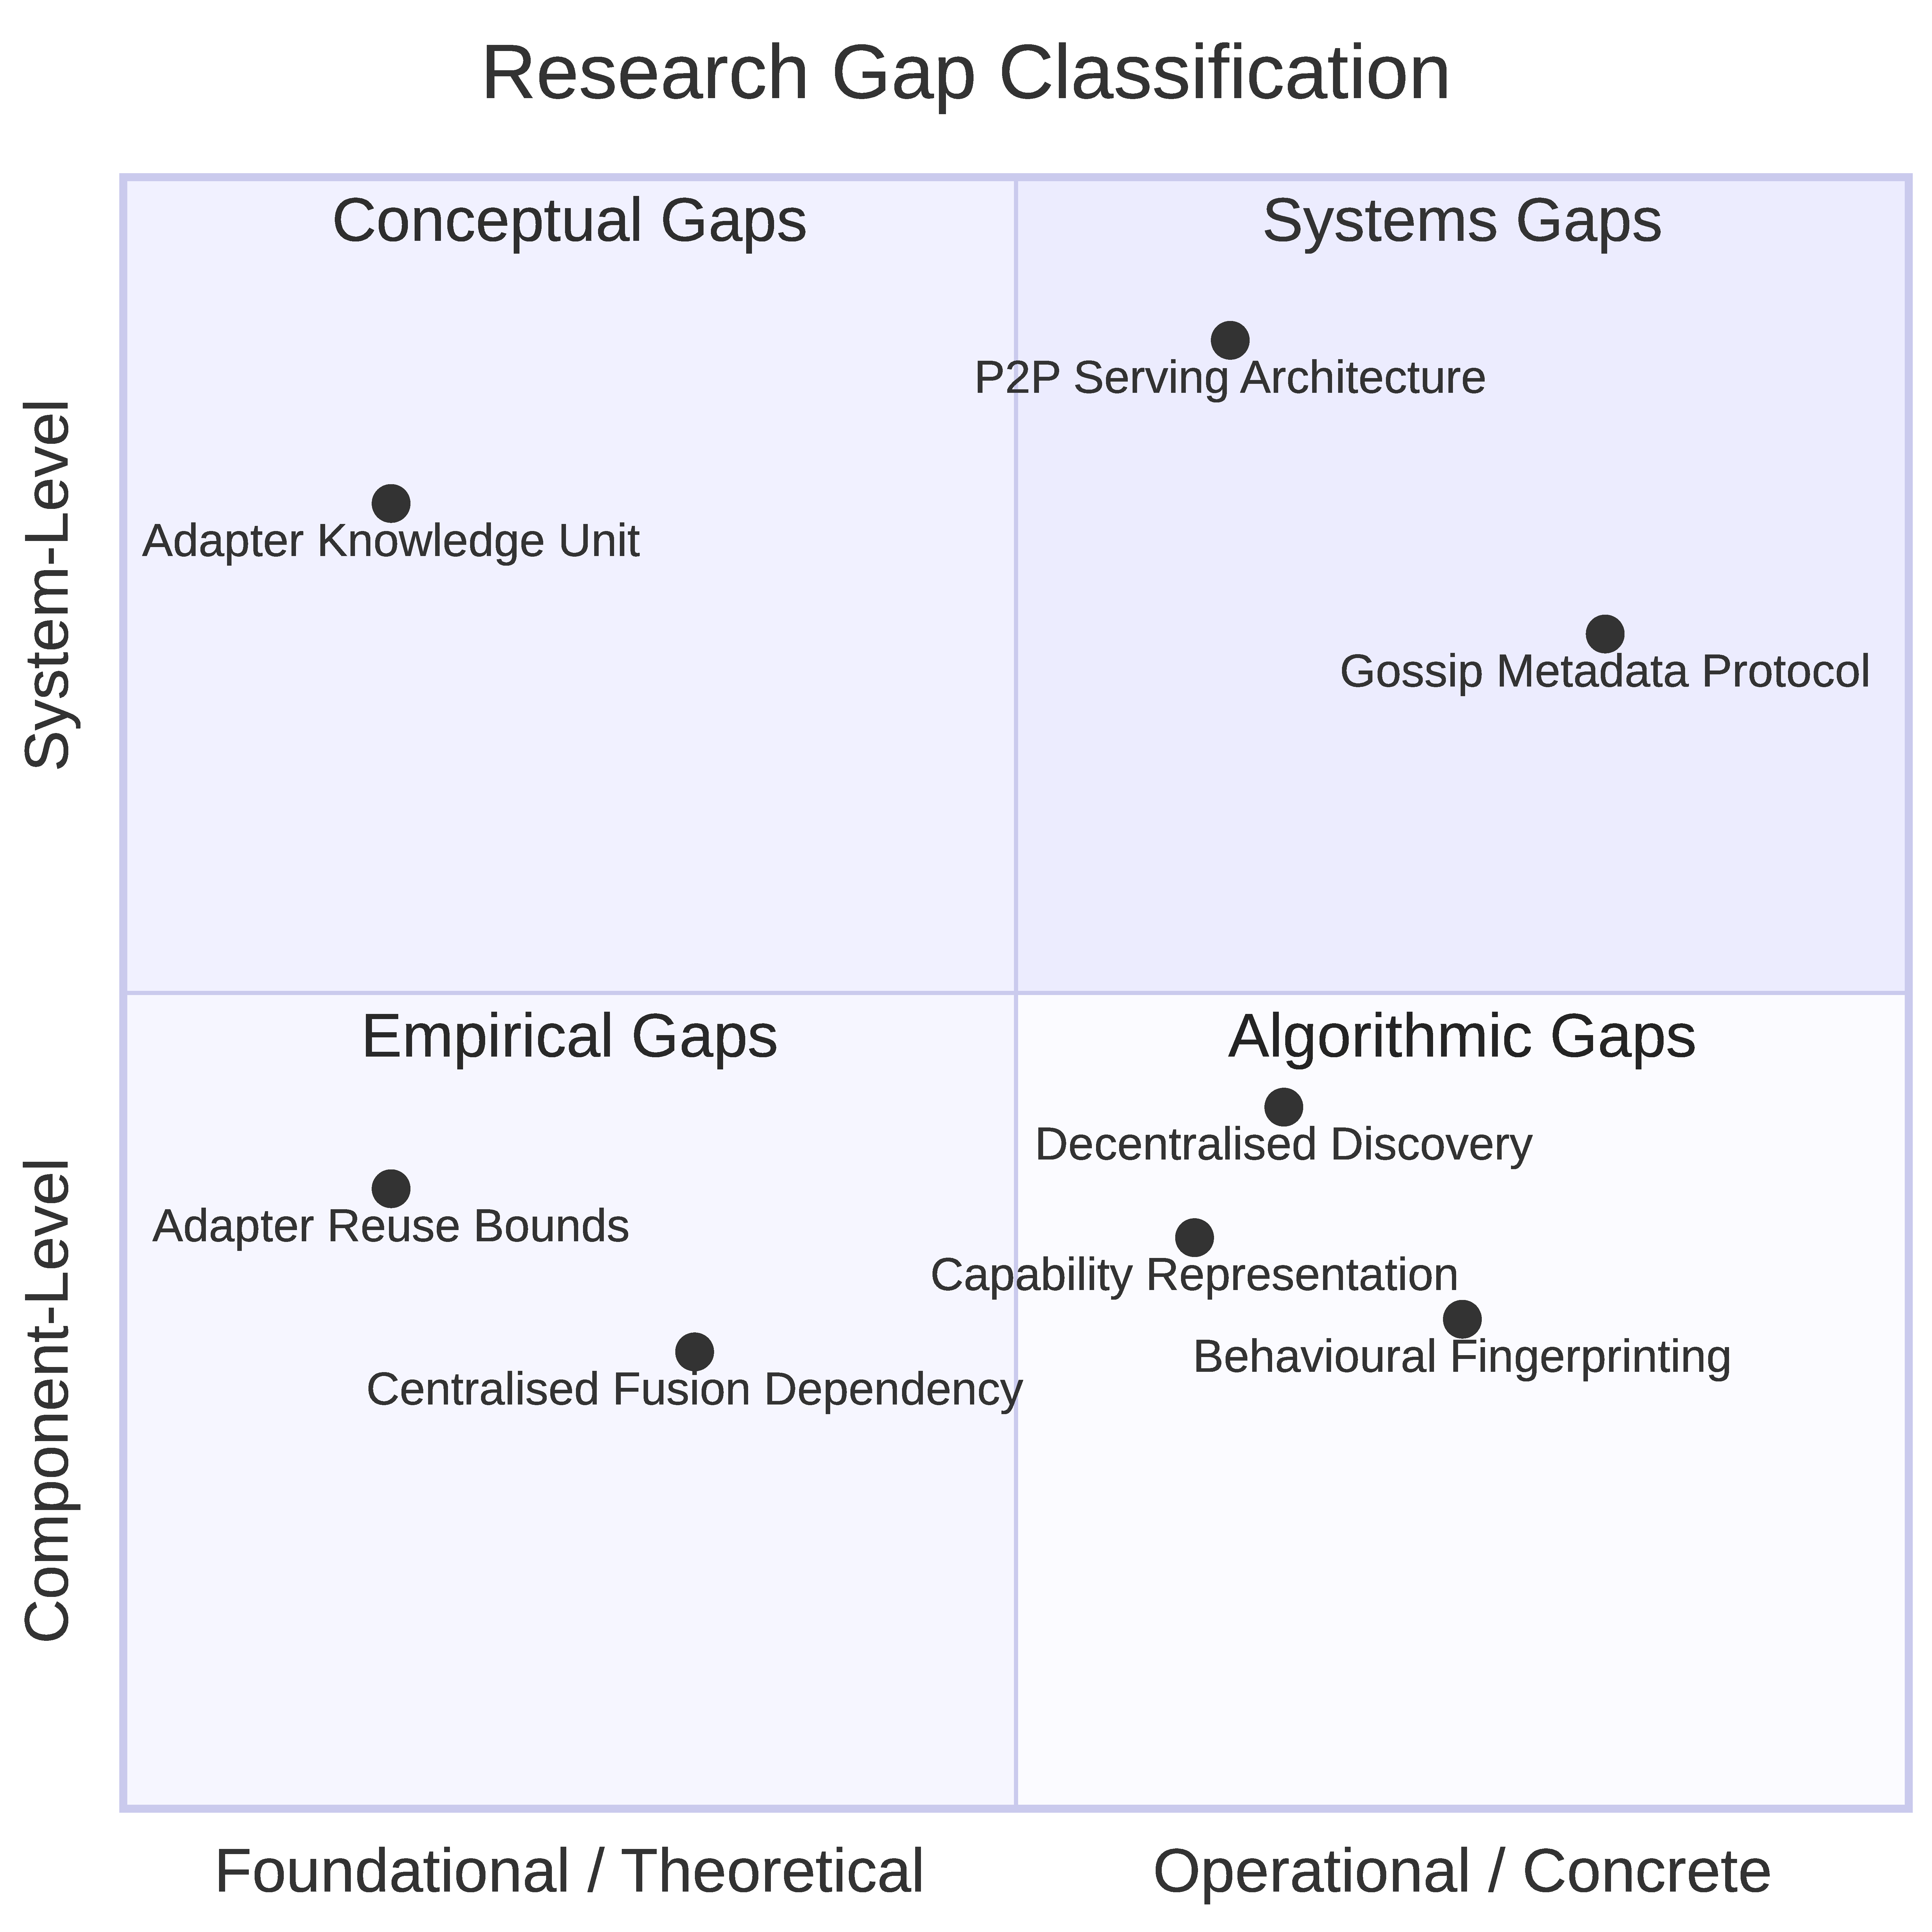
\includegraphics[width=0.85\linewidth]{figures/fig_gap_quadrant.pdf}
  \caption{Research gap taxonomy: gaps identified from the concept matrix classified
         into four quadrants by type of work required (foundational/operational)
         and scope of effect (system-level/component-level).}
  \label{fig:fig_gap_quadrant}
\end{figure}

The top-left quadrant contains the conceptual gap: the reviewed literature does not appear to frame adapters as autonomous, transferable knowledge units within a P2P context. This gap is foundational in the sense that the algorithmic and systems gaps below presuppose such a framing.

The top-right quadrant holds the systems gaps: concrete, implementation-level 
questions whose resolution would shape the overall behaviour of a decentralised setting, 
in contrast to the component-level gaps below.

The bottom-right quadrant contains three algorithmic gaps: a discovery protocol,
a structural representation, and a behavioural representation, because the
discovery problem decomposes naturally into these three distinct components.

The bottom-left quadrant holds two empirical gaps that require theoretical derivation
and experimental validation before they can be resolved.

\paragraph{Conceptual gap: adapters as atomic P2P knowledge units.}
Existing literature treats adapters either as fine-tuning artefacts (PEFT literature)
or as parameters to aggregate (FL literature), but no reviewed work defines adapters as autonomous, transferable knowledge units capable of being \textit{proposed}, \textit{evaluated}, and \textit{exchanged} by independent peers without any shared training context. The concept of an adapter as a first-class knowledge commodity: with an identity, a provenance, a capability description, and a trust score does not appear in the reviewed literature. This conceptual gap defines an open research question: what
properties must an adapter possess (beyond its weight matrices) to
function as an exchangeable knowledge unit between autonomous peers, and how
should identity, provenance, and capability be represented?

\paragraph{Algorithmic gaps: discovery protocol, capability embeddings, behavioural fingerprints.}
Three algorithmic gaps follow from the missing discovery dimension in Table~\ref{tab:concept_matrix}.
\begin{itemize}
  \item \textbf{Adapter discovery protocol.} No reviewed system provides a protocol for a node to discover, across a P2P network, which peers hold adapters relevant to a given query without contacting a central registry. This gap
    defines the first open algorithmic question: can DHT-based infrastructure,
    proven at scale in systems such as Kademlia \cite{MaymounkovKademlia2002},
    support adapter discovery at the capability level rather than the identifier level?
  \item \textbf{Adapter capability embeddings.} Effective discovery requires
    a compact representation of what task a given adapter performs, computable from
    the adapter's weight matrices alone (without access to training data).
    This raises an open representation question: do the weight-space properties
    of trained adapters carry sufficient task-level signal to enable
    similarity-based retrieval without access to training data or task labels?
  \item \textbf{Behavioural fingerprints.} Capability embeddings based on
    weight spectra may not capture functional behaviour under distribution shift.
    This raises a complementary open question: can probe-set
    outputs provide a functional description of adapter behaviour that is
    more robust to distribution shift than structural weight-space representations?
\end{itemize}

\paragraph{Systems gaps: P2P adapter exchange architecture and gossip-based dissemination.}
The systems literature (Section~\ref{sec:inference_systems}) demonstrates efficient multi-adapter serving within a single administrative domain, but no reviewed architecture addresses the P2P setting with autonomous nodes. Two systems gaps remain open.
\begin{itemize}
  \item \textbf{P2P adapter exchange architecture.} No reviewed work proposes a P2P architecture for adapter exchange without central infrastructure. This gap defines the primary
    systems-level open question: what communication and storage primitives are
    necessary and sufficient for adapter sharing across autonomous peers without
    any central scheduler or repository?
  \item \textbf{Gossip-based adapter metadata dissemination.} A related open question
    is whether gossip-based propagation, known to achieve network-wide awareness
    in $O(\log N)$ rounds \cite{OrmandyGossip2013}, is sufficient for adapter
    metadata dissemination under realistic peer churn and bandwidth constraints.
\end{itemize}

\paragraph{Empirical gaps: reuse bounds and decentralised fusion.}
Two empirical gaps remain open in the reviewed literature.
\begin{itemize}
  \item \textbf{Adapter reuse quality under non-IID distributions.} The federated PEFT literature has demonstrated that adapter aggregation degrades under heterogeneous data distributions \cite{ZhangFedPETuning2023, Li2020FedProx}, but no reviewed work has derived bounds on adapter reuse quality as a function of distribution distance between the contributing peer's training distribution and the requesting peer's query distribution. The domain adaptation literature establishes that such a bound is theoretically tractable (Ben-David et al.~\cite{BenDavid2010} ground similar degradation guarantees in divergence measures between source and target distributions), but this result has not been instantiated for the adapter reuse setting, where the source distribution is unknown to the receiving peer and adapter rank introduces an additional capacity constraint. Formally characterising this degradation as a function of distribution distance and adapter rank remains an open theoretical question.
  
  \item \textbf{Centralised fusion dependency.} AdapterFusion \cite{Pfeiffer2021fusion}
    requires a centralised fusion training step that is incompatible with a fully
    P2P setting. This raises the open architectural question: can probe-based
    local estimation replace centralised fusion training without unacceptable
    performance loss, and under what conditions on probe set size and adapter
    diversity does the approximation degrade?
\end{itemize}

\subsection{Research Gap Map}
\label{sec:synthesis_gap:gap_map}

Table~\ref{tab:gap_map} consolidates the gaps identified in this review,
organised by quadrant, with the concept matrix dimensions they address
and the open research question each gap defines. This map is the principal
analytical deliverable of the SLR: a structured account of which gaps remain
open \emph{within the reviewed corpus} and what a future research programme
in this direction must resolve.

\begin{table}[H]
\centering
\caption{Research gap map: identified gaps grouped by quadrant, with evidence
         base, unaddressed concept matrix dimensions, and open research question.}
\label{tab:gap_map}
\setlength{\tabcolsep}{4pt}
\footnotesize
\begin{tabular}{p{2cm}p{3.5cm}p{1.5cm}p{2cm}p{4cm}}
\toprule
\textbf{Quadrant} &
\textbf{Gap Description} &
\textbf{Evidence} &
\textbf{Dimensions Unaddressed} &
\textbf{Open Research Question} \\
\midrule
Conceptual &
  Within the reviewed corpus, no work yet frames adapters as autonomous,
  transferable knowledge units with identity, provenance, and capability in a
  P2P context &
  G0--G6 &
  Adapter exchange + P2P &
  What properties must an adapter possess to function as an exchangeable
  knowledge unit between autonomous peers? \\
\midrule
\multirow{3}{*}{Algorithmic} &
  No protocol has been identified for locating task-relevant adapters across a P2P network
  without a central registry &
  G3, G4 &
  Discovery &
  Can DHT-based lookup support capability-level adapter discovery at scale? \\[4pt]
  &
  No reviewed method derives a compact, data-free representation of adapter functional
  capability from weights alone &
  G2, G5 &
  Discovery &
  Do weight-space properties of adapters carry sufficient task-level signal
  for similarity-based retrieval? \\[4pt]
  &
  No reviewed method provides a functional, behaviour-based adapter descriptor robust
  to distribution shift &
  G2, G4 &
  Discovery &
  Can probe-set outputs provide functional capability descriptions more robust
  than structural weight representations? \\
\midrule
\multirow{2}{*}{Systems} &
  No P2P architecture has been proposed for adapter exchange without central infrastructure &
  G3, G4 &
  P2P + No central coord. &
  What communication and storage primitives are necessary and sufficient for
  decentralised adapter sharing? \\[4pt]
  &
  No gossip-based protocol has been identified for adapter metadata dissemination across
  a dynamic peer population &
  G3, G6 &
  P2P + No central coord. &
  Is gossip propagation sufficient for adapter metadata under realistic churn
  and bandwidth constraints? \\
\midrule
\multirow{2}{*}{Empirical} &
  No theoretical bounds have been derived for adapter reuse quality as a function of
  distribution distance between peers &
  G3, G6 &
  Adapter exchange + P2P &
  Under what distributional conditions does adapter reuse degrade to an
  unacceptable degree, and can this be bounded formally? \\[4pt]
  &
  All reviewed composition methods require centralised training data for the
  fusion step, incompatible with P2P operation &
  G2, G5 &
  Multi-task fusion &
  Can probe-based local weight estimation replace centralised fusion training
  without unacceptable performance loss? \\
\bottomrule
\end{tabular}
\end{table}

\subsection{Research Directions and Open Problems}
\label{sec:synthesis_gap:directions}

The gap map in Table~\ref{tab:gap_map} addresses the overarching research question posed in Section~\ref{sec:introduction}: the reviewed literature does not yet provide all of the building blocks that a fully decentralised adapter-based inference setting would require. The identified gaps span four distinct research dimensions, each demanding different methodological commitments.

The conceptual gap is the prerequisite. Until adapters are treated as
first-class knowledge units with explicit capability representations, the
algorithmic and systems gaps cannot be meaningfully addressed, because there
is no well-defined object to discover, route, or exchange. The algorithmic
gaps are the most numerous and decompose naturally into a discovery protocol
question, a structural representation question, and a functional representation
question. The systems gaps require architectural design and empirical validation
at the infrastructure level. The empirical gaps require formal theoretical work
on distribution shift and controlled experimental comparison of fusion strategies.

Taken together, these findings support the assessment that decentralised adapter-based
inference is a coherent research direction, theoretically motivated by converging evidence
from adjacent fields and as yet empirically unexplored. The evidence base assembled in this review indicates that
the constituent fields: PEFT, P2P systems, and multi-tenant serving
each contribute necessary but individually insufficient pieces. The gap map in 
Table~\ref{tab:gap_map} provides a structured account of that intersection 
and the open questions it raises.